\chapter{A Living Database}\label{ch:livingdb}

\section*{Introduction}
\addcontentsline{toc}{section}{Introduction}

Every chapter so far has treated the database as a fixed thing sitting
underneath the agent: a schema to design, a set of tables to query. It
never actually is one. From the first tick after the server starts, a
separate process is quietly rewriting both databases underneath
whatever the agent is doing --- shifting KPIs, opening and healing
service incidents, accumulating usage, recomputing churn scores,
occasionally creating a brand-new subscriber out of nowhere. The agent
in the next chapter is built entirely around the assumption that this
is true: that the world it is answering questions about is not sitting
still, and that nothing it has already said can be trusted to still be
correct a few minutes later. Before getting into what the agent can do
with that world, this chapter covers what the world itself actually
does on its own.

\section{Why a Static Database Was Never Going to Be Enough}
The database created from Chapter 
The synthetic databases from Chapter~\ref{ch:database} gave the project
something to query, but a database that only changes when someone re-runs a
generation script is just a snapshot. Real networks don't sit still, so ours
shouldn't either. There's a less obvious reason too: if the numbers never move,
an agent that quietly memorized its first answer looks exactly as correct as one
that queries the database honestly every time. A moving target is the only way
to tell those two apart --- which is what \texttt{db\_simulator.py} is for.

\section{The Tick Loop}

\texttt{db\_simulator.py} runs as its own long-lived process, entirely
separate from the chat server, and advances the environment forward on
a fixed schedule --- one \emph{tick} every few minutes. Each tick walks
through a set of update functions, and each one touches a different
slice of the two databases:

\begin{itemize}
    \item \textbf{KPIs and alarms} --- network performance metrics
    (throughput, latency, drop rate) get nudged, faults get raised on
    cells, and the two are wired to each other in both directions
    (Figure~\ref{fig:ch4-alarms}).
    \item \textbf{Usage} --- this updates montly data and voice usage for a rotating
    number of subscribers, relatively like real usage would build up gradually over
    the course of a month, rather than getting an impulse.
    \item \textbf{Churn rescoring} --- every affected subscriber's
    churn risk gets calculated again, based on their latest activities, and 
    how network KPIs affect thenm, not left stale from whenever it was last 
    calculated.
    \item \textbf{New subscribers} --- occasionally, the database may get or lose 
    a new subscriber, it gets created from scratch and added to both databases at once, so the 
    50{,}000 isn't a fixed number either.
    \item \textbf{The calendar} --- the simulator keeps its own notion
    of ``today,'' and that notion advances tick by tick independently
    of the real-world date. A month can complete and roll over inside
    the simulation without the actual calendar moving at all.
\end{itemize}

% =====================================================================
% SCREENSHOT NEEDED --- figures/ch4-alarms.png
% Where: analytics dashboard (localhost:8002), Network section.
% What to capture: the KPI trend chart together with the active alarms
% list/table, showing both a chart (built from kpis_daily) and a set of
% currently-raised alarms in the same view.
% =====================================================================
\begin{figure}[H]
\centering
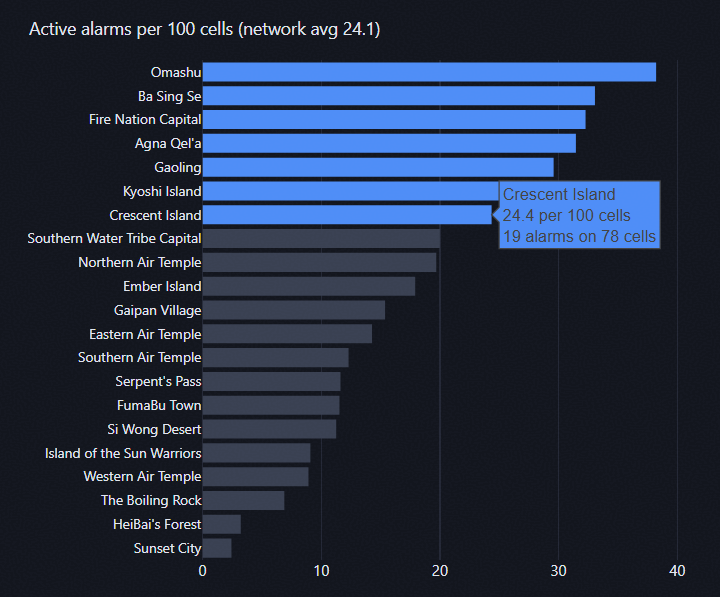
\includegraphics[width=0.85\textwidth]{figures/ch4-alarms.png}
\caption{Active alarms per 100 cells by region, from live simulator data.
Omashu leads once normalized.}

\label{fig:ch4-alarms}
\end{figure}

These updates aren't dramatic on their own, but with enough time, it accumulates a more 
interesting result, asking the agent the same question a minute apart won't change much,
but an hour, it'll show significant change, something a static database could never offer.


% =====================================================================
% SCREENSHOT NEEDED --- figures/ch4-simulator-tick.png
% Where: terminal running db_simulator.py directly (python db_simulator.py).
% What to capture: a few consecutive tick log lines showing the kind of
% updates it applies each cycle (KPI updates, alarms, churn rescoring,
% new-incident lines, etc.) --- enough to show it is a continuously
% running process ticking forward, not a one-shot script.
% =====================================================================
\begin{figure}[H]
\centering
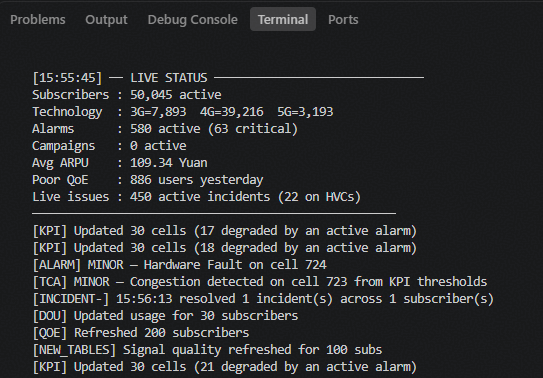
\includegraphics[width=0.85\textwidth]{figures/ch4-simulator-tick.png}
\caption{\texttt{db\_simulator.py} running its tick loop, continuously updating
both databases while the agent stays live.}
\label{fig:ch4-simulator}
\end{figure}

\section{Live Service Incidents: Open, Spread, Heal}

The most involved piece of the simulator is not a background metric
drifting slightly --- it is a full incident lifecycle, built so the
agent can be asked something like ``do we have any high-value
customers having streaming issues right now'' and get a real, current,
truthful answer.
Every incident lives in an \texttt{experience\_incidents} table, it has a root 
cause, an affected service, a severity and a full timestamp trail. But one incident
can't really be a lone flag on a row: opening one also lays down a run of poor 
QoE scores for that service, a matching service-interruption, and, if it's serious enough,
a customer complaint is also filed. 
. Asking the agent to explain \emph{why} a
customer's experience looks bad is meant to hold together as a story,
not just a single suspicious number.

\subsection{Blast Radius: Not Every Fault Hits One Customer}

An early version of this feature made every incident purely
per-customer, and it produced a result that did not survive a second
look: a ``critical power failure at a site'' that supposedly affected
exactly one subscriber, when that site was actually serving over fifty
people. The fault itself was real and correctly reported by the agent
--- the problem was in the data, not the reasoning built on top of it,
which is precisely why it is worth naming here rather than in the next
chapter: it was a modeling gap in the simulator, not a mistake by the
agent.

The fix was to give every incident a defined \emph{scope}, matching how
that class of fault actually behaves in a real network:

\begin{table}[H]
\centering
\small
\begin{tabular}{@{}p{3.1cm}p{4.9cm}p{5.4cm}@{}}
\toprule
\textbf{Scope} & \textbf{Who it affects} & \textbf{How the simulator picks it} \\
\midrule
\textbf{Site}\newline{\footnotesize power failure, site outage}
& Every active subscriber on every cell at that site
& \(\sim\)2\% of new incidents --- an outage that big is rare \\
\addlinespace
\textbf{Cell}\newline{\footnotesize congestion, backhaul degradation, interference}
& Every active subscriber on that cell
& Weighted toward busier cells, where congestion actually happens \\
\addlinespace
\textbf{Subscriber}\newline{\footnotesize throttling, DNS or CDN hiccup, dropped VoLTE bearer}
& One customer
& Biased toward high-value subscribers \\
\bottomrule
\end{tabular}
\caption{Incident scopes and how the simulator selects them.}
\label{tab:incident-scopes}
\end{table}

``High-value'' here is not a fixed ARPU threshold but the top decile of the live
distribution, re-tested as revenue moves --- so the label keeps meaning
something even as ARPU drifts

Once a site- or cell-scoped incident fires, every subscriber caught in
its blast radius gets a consistent snapshot of the incident attached to
their record --- so a question filtered to high-value customers only
returns the high-value customers genuinely inside that radius, not
everyone the fault happened to touch. A power failure at a site serving
mostly bronze-tier subscribers in a poorer part of the fictional map
and one serving mostly platinum subscribers in a wealthier one are the
same fault with completely different commercial urgency, which is
exactly the distinction a purely per-customer model could never have
produced.

\subsection{Self-Healing}

An incident does not sit open forever. Every tick, a separate resolution
pass checks every active incident against the \texttt{expected\_}
\texttt{resolution\_at} timestamp it was given at open, and closes
anything past due: status flips to resolved, \texttt{resolved\_at} gets
stamped, and any linked complaint gets marked resolved too. The row
itself is never deleted, so a question like ``what happened to this
customer at 14:32 today'' still has a real answer to give hours or days
later --- the incident heals, but the history of it having happened
does not disappear with it.

\section{Alarms That Actually Mean Something}

The blast-radius problem had a sibling that hid for much longer. Alarms
and KPIs both looked fine on their own --- the alarms table filled up,
the KPI numbers moved --- so neither invited a second look. But the issue is 
that they never linked/synced with each other, this means that each tick raised
an alarm on a cell picked randomly, wrote the row, and stopped there, while 
the KPI generator rolled its own seperate dice and never read the alarms this table.
The giveaway was clear in the data though: cells carrying an active \emph{critical}
alarm measured a slightly \emph{lower} drop rate than cells with no alarm at all.
This of course made no sense and had to be fixed. And since cells were picked from the whole network rather than
the parts of it serving people, 62\% of alarms sat on cells with zero
subscribers on them.


Fixing it meant wiring the two together in both directions, because
real faults work both ways. Equipment faults --- a power failure, a
hardware fault, a backhaul link going down --- announce themselves, and
the degraded counters follow as a consequence. Performance faults are
the reverse: congestion, interference and coverage holes have no box to
raise a flag, and the only way anyone finds out is by watching the
counters cross a threshold, which is what a real network management
system calls a threshold-crossing alert. So a raised fault now degrades
the cell it sits on --- each fault type hitting the metric it would
actually hit, scaled by severity --- and opens real incidents for the
customers on that cell if it is serious enough, feeding the same
evidence trail and churn coupling described above. Running the other
way, a detector reads each cell-day and raises the alarm those numbers
deserve.

One detail there is worth keeping, because the obvious approach fails
quietly. Thresholds need to relative to the technology and not absolute: a 
1.9\% drop rate is a broken 5G cell and a completely ordinary 2G one. A flat ``
drop rate above 2\%'' rule currently flags 188 2G cells, 45 for 3G and 50 for 
4G, and not one of those 2G is under an alarm, while the 4G ones, all of them are 
under an alarm. So the rule works and does find real faults, and then buries them
under nearly four times as many cells whose only crime is being 2G.
Every threshold is therefore expressed against that technology's own
healthy baseline.

One bug is worth admitting: the KPI update function had never written a single
row. Its upsert depended on a uniqueness constraint the table didn't have, the
database helper swallowed the error, and the function went on reporting success
every tick. The helpers now print real errors instead of retrying past them.
With that fixed, cells under an active alarm run 1.4 to 2.1 times the drop rate
of clean cells, and 1{,}089 of 1{,}099 active alarms sit on a cell that actually
serves somebody.


\section{Churn Tracks the Live World, Not Just Usage}

Churn risk here is the sum of two parts, computed separately on purpose. The
first is a baseline from a subscriber's own commercial behaviour --- spend
falling against their own history, bills going unpaid, usage tailing off, a short
tenure. The second is a penalty from what is happening to them on the network
right now. Chapter~\ref{ch:eval} covers how that baseline is computed and why it
ended up as an explainable scorecard rather than the machine-learning model
originally trained for it.

The reason for splitting them is that a baseline built from monthly commercial
history has no way of reacting to something happening to a customer
\emph{today}. The live incident log closes that gap: every affected subscriber
is rescored the moment an incident opens against them, with a penalty added on
top of the baseline, driven by how many active incidents and unresolved
complaints they currently have. Once the incident heals, the next rescoring pass
lets that penalty relax back down.

So a platinum subscriber sitting on a comfortable, low-risk baseline can be
pushed into a genuinely elevated risk band for as long as their streaming
service is actually degraded, and settle back down once it recovers --- churn
risk that tracks the live state of the world, rather than a number computed once
and left to go stale. The two halves are kept strictly separate: the baseline
never reads incidents, and the penalty never reads commercial history, so
neither signal is counted twice.

\section{Seeing It on the Map}
The coverage map associated to the work is not just a static look, it
represents multiple things: the cell site locations, showing density in 
certain cities, as well as current alarms, clicking on a ring will immediately
prompt the agent to investigate the said alarm, searching up root cause as well as suggesting solutions.


% =====================================================================
% SCREENSHOT NEEDED --- figures/ch4-map-flash.png
% Where: chat UI (localhost:8000), Coverage tab in the snapshot panel.
% What to capture: the map with at least one pulsing incident ring
% visible, ideally with the hover tooltip open showing the site/service/
% severity details. If you can catch the "Issues only" toggle active
% too, even better --- otherwise a normal view with rings is enough.
% =====================================================================
\begin{figure}[H]
\centering
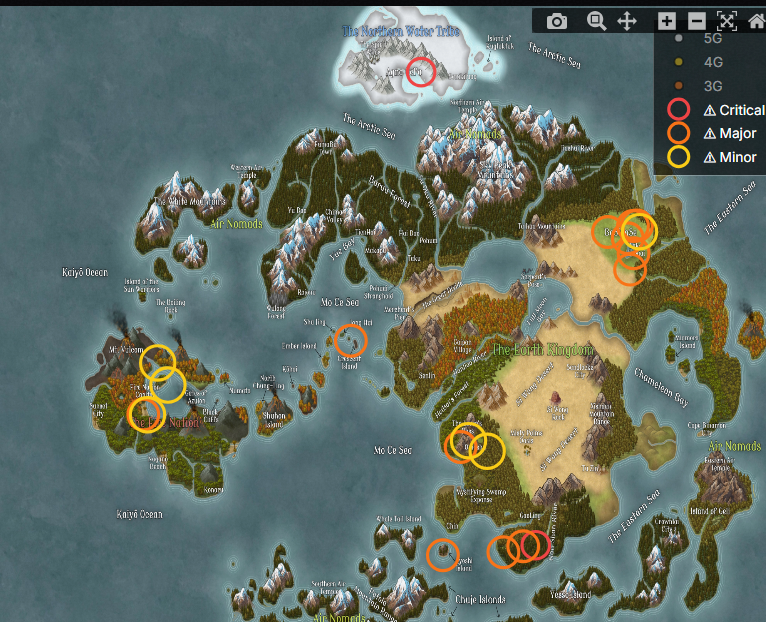
\includegraphics[width=0.85\textwidth]{figures/ch4-map-flash.png}
\caption{The coverage map flashing a live incident, colored and pulsing
by severity, driven directly by the active rows in
\texttt{experience\_incidents}.}
\label{fig:ch4-map-flash}
\end{figure}

\section{The Partial-Month Gotcha}

Because monthly usage figures accumulate tick by tick over the course
of a simulated month rather than existing fully formed from day one,
there is a real and slightly counterintuitive consequence worth naming
directly: a question asked on the second day of a new simulated month
legitimately returns a much smaller number than the exact same question
asked on the last day of the previous one. When read in isolation, a ``
top data user this month'' answer of a few gigabytes early in a cycle 
can look like the agent got it wrong, when in reality, it was the correct 
answer, just not logically. This came up directly while testing: an 
answer citing a small usage figure for a specific subscriber 
looked like the number was hallucinated at first glance, but checking the 
database it was correct, as the month had just begun.  Knowing the data is
genuinely live --- not stale, not wrong, just incomplete for the
current period --- is what keeps a correct answer from being misread
as a bug.

\section*{Conclusion}
\addcontentsline{toc}{section}{Conclusion}

This chapter covered the piece of the project that everything else
quietly depends on: a database that never actually holds still.
\texttt{db\_simulator.py} advances KPIs, usage, and the subscriber base
tick by tick, but the real weight of the chapter is the incident
lifecycle built on top of it --- faults that open with a real cause, a
proportionate blast radius instead of a flat per-customer model, and a
resolution path that lets them heal on their own, all of it feeding
directly into churn scoring and the live coverage map. None of this
exists for its own sake. It exists so that the agent, covered in the
next chapter, cannot get away with memorizing an answer and repeating
it --- every claim it makes has to survive being checked against
whatever the database currently says, because the database it is
reading from is not the same one it was reading from five minutes ago.
